\noindent\begin{tabular}{@{\hspace{0.0em}}c@{\hspace{0.0em}}c@{\hspace{0.0em}}}
With & Without\\
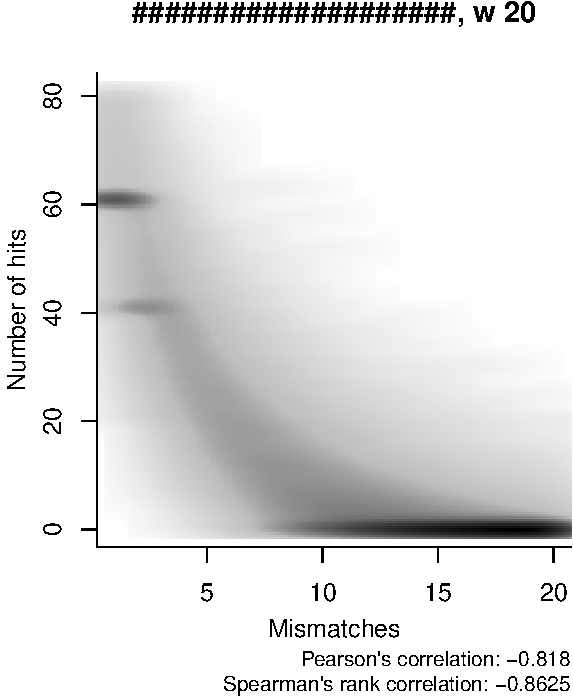
\includegraphics[width=0.49\linewidth]{images/3.3/Myco-w20-cont-hit-scatter-crop.pdf} &
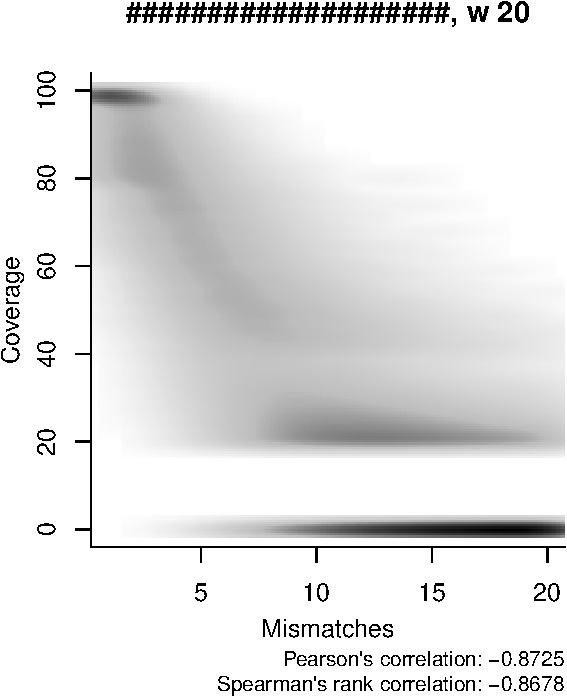
\includegraphics[width=0.49\linewidth]{images/3.3/Myco-w20-cont-cover-scatter-crop.pdf} \\%[2em]
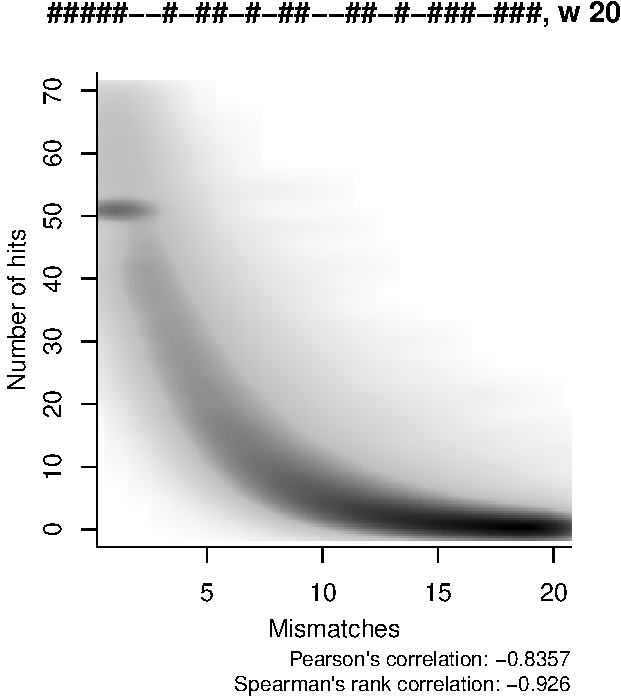
\includegraphics[width=0.49\linewidth]{images/3.3/Myco-w20-spaced-hit-scatter-crop.pdf} &
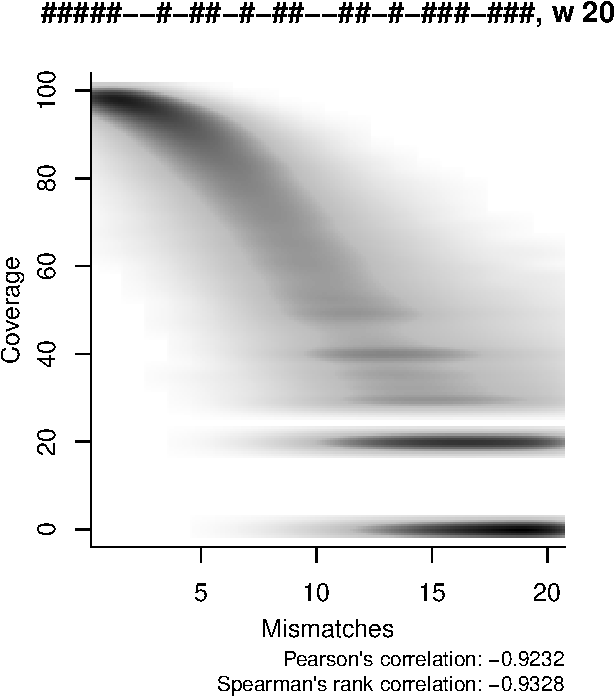
\includegraphics[width=0.49\linewidth]{images/3.3/Myco-w20-spaced-cover-scatter-crop.pdf} \\%[2em]
%\begin{sideways}{\makebox[0.32\linewidth][c]{Flank of a giraffe}}\end{sideways} & 
%\includegraphics[width=0.40\linewidth]{candidates_giraffes_flank_bg}&
%\includegraphics[width=0.40\linewidth]{candidates_giraffes_flank_no_bg}\\
\end{tabular}

% 
% \begin{figure*}
% 	%\centering
% 	\begin{subfigure}[b]{0.47\textwidth}
% 		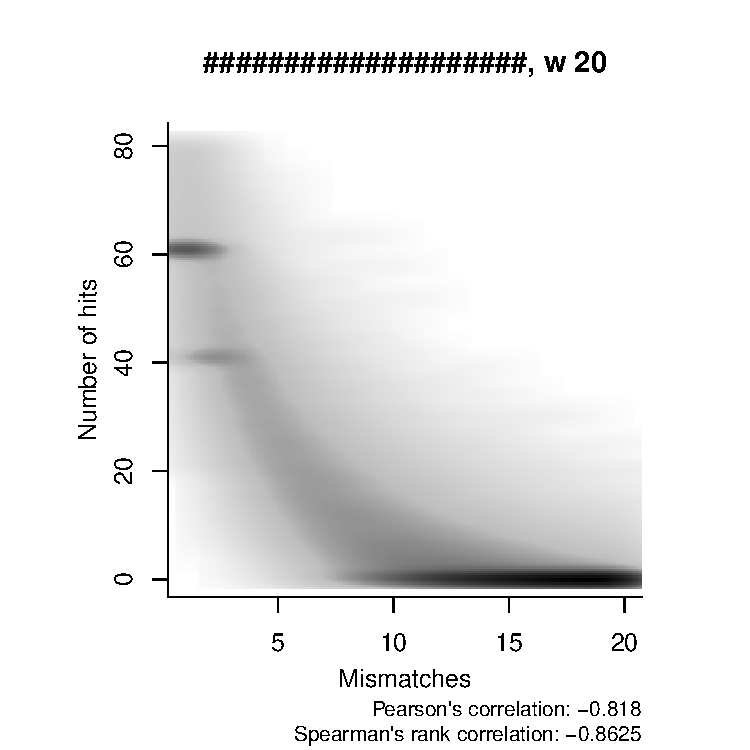
\includegraphics[width=\textwidth]{images/3.3/Myco-w20-cont-hit-scatter.pdf}
% 		\label{weight-20-cont-hit-scatter}
% 	\end{subfigure}
% 	~
% 	\begin{subfigure}[b]{0.47\textwidth}
% 		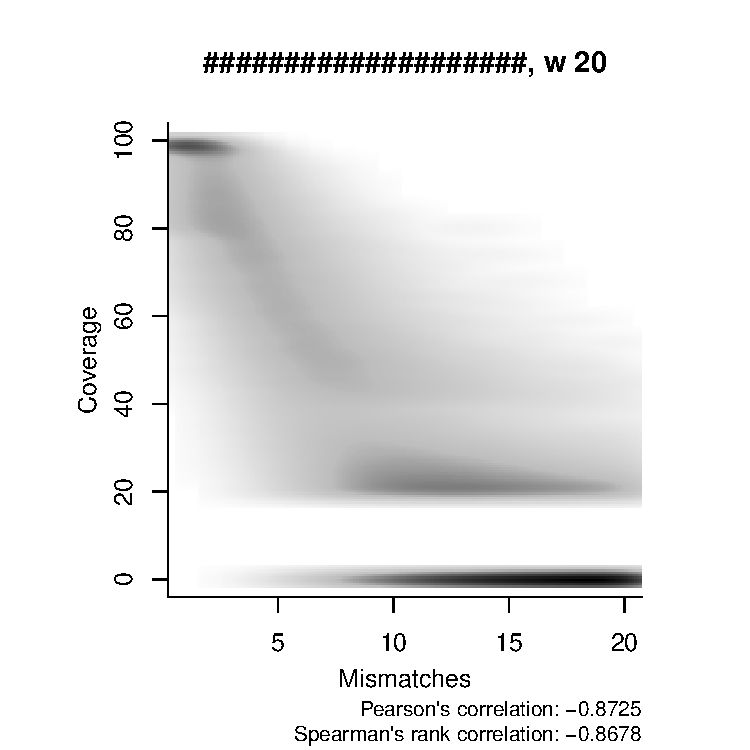
\includegraphics[width=\textwidth]{images/3.3/Myco-w20-cont-cover-scatter.pdf}
% 		\label{weight-20-cont-cover-scatter}
% 	\end{subfigure}
% 
% 	\begin{subfigure}[b]{0.49\textwidth}
% 		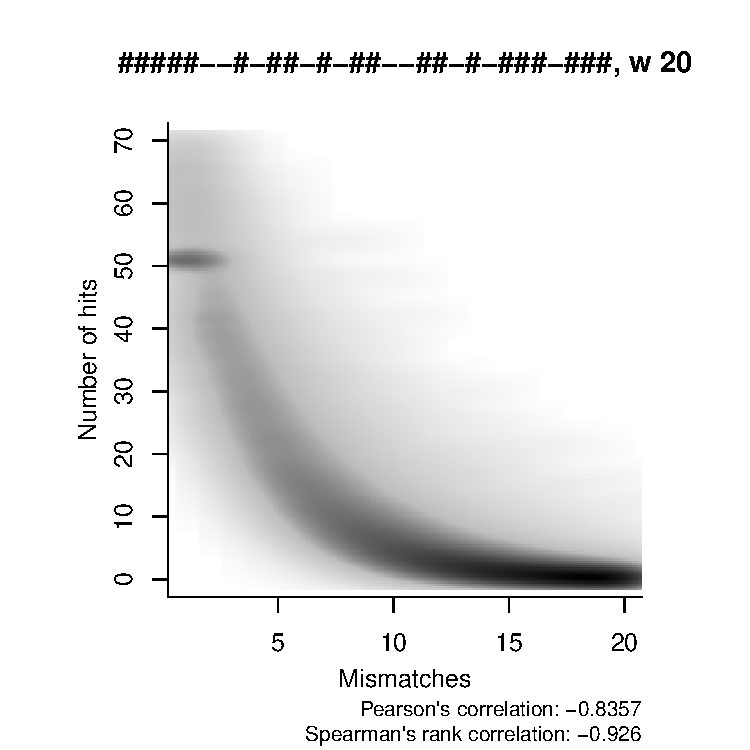
\includegraphics[width=\textwidth]{images/3.3/Myco-w20-spaced-hit-scatter.pdf}
% 		\label{weight-20-spaced-hit-scatter}
% 	\end{subfigure}
% 	~	
% 	\begin{subfigure}[b]{0.49\textwidth}
% 		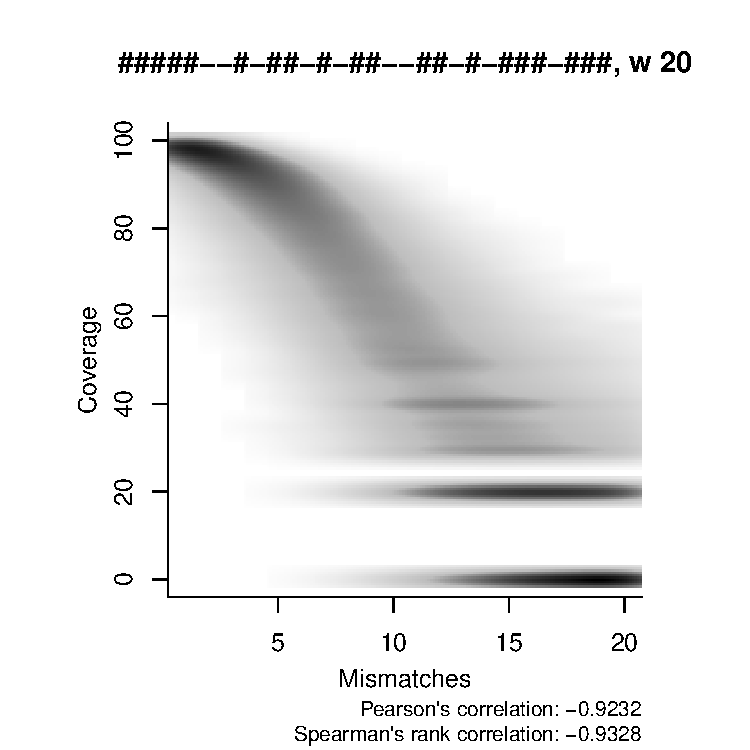
\includegraphics[width=\textwidth]{images/3.3/Myco-w20-spaced-cover-scatter.pdf}
% 		\label{weight-20-spaced-cover-scatter}
% 	\end{subfigure}
% 	
% 	\caption{Hit number (left plots) and coverage (right plots) depending
% 	on the number of mismatches in randomly generated reads. Seed is
% 	shown above the plot, and Spearman's and Pearson's correlations are
% 	shown below. Grayscale shows the density of
% 	reads. Experiments made on {\em M.tuberculosis} 
% 	genome. \label{clouds}}
% \end{figure*}
